\section{Background}

This section will cover some of the fundamental concepts both in quantum mechanics and classical computing which are required for understanding this paper. 
Finally the DiVincenzo criteria will be introduced which is five objectives that should be met by any system in order to be an effective large scale quantum computer. 

\subsection{Fundamentals of Classical Computing}
Quantum computers are an extension of the founding principles of classical computation, which take advantage of quantum mechanical phenomena. Therefore, in order to understand how to build a quantum computer, it is beneficial to have a strong understanding of a classical computer's basic components. In order to build a functioning quantum computer, every fundamental feature described in the sections below must have an analogous, albeit quantum, implementation.
\subsubsection{What is a bit? Or a nibble, or even a byte...}
In computing the smallest unit of information is known as a bit, and can take a value of 1 or 0. This is because computers work in a binary number system as opposed to the decimal system one learns as a child, where a single digit can take values from 0 to 9. The major motivation behind this was for ease of implementation; it is much easier to create a switch that can be on or off than one that has 10 different positions. 

Individual bits don't allow us to represent much, however, we can chain them together to represent larger and larger numbers. We call a group of four bits a nibble, and more commonly known is a group of eight - a byte. Figure \ref{fig:BINARY} illustrates how six bits are combined to make the number 45, where digits further to the left show contributions from higher powers of 2.
\begin{figure}[H]
    \centering
    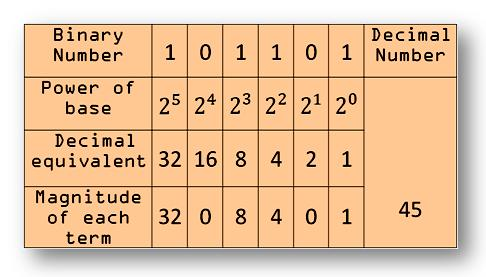
\includegraphics[width=0.6\textwidth]{images/binary.jpg}
    \caption{A table illustrating how to convert the binary number 101101 into its decimal equivalent, 45 \cite{binary}}\label{fig:BINARY}
\end{figure}

\subsubsection{How is a bit physically stored?}
Use figure here
\subsubsection{Gates - Manipulating bits}
Clearly bits can be used to represent different values or states, however, it is their processing and manipulation which allows for computation. Gates are components which take one or more bits as input, and output a single bit with a state dependent on the input values. Figure \ref{fig:ANDGATE} shows the diagrammatic symbol for an AND gate along with all of its possible outputs. The AND gate will output 1 only if both of its inputs are also 1 (otherwise it outputs 0).
\begin{figure}[H]
    \centering
    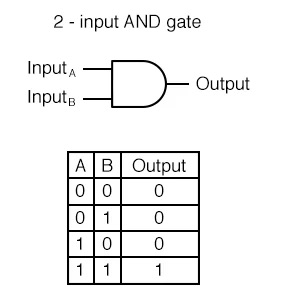
\includegraphics[width=0.4\textwidth]{images/andgate.jpeg}
    \caption{The circuit symbol for an AND gate, along with a truth table of all possible outputs for two inputs, A and B. \cite{andgate}}\label{fig:ANDGATE}
\end{figure}

There are many other gates, such as the NOT which takes a single bit as input and outputs a bit with the opposite state. The important point to highlight is that gates provide building blocks for computation.

\subsubsection{Computation - Many gates}
Computer algorithms can be boiled down to passing bits through a circuit of different gates. 
\begin{figure}[H]
    \centering
    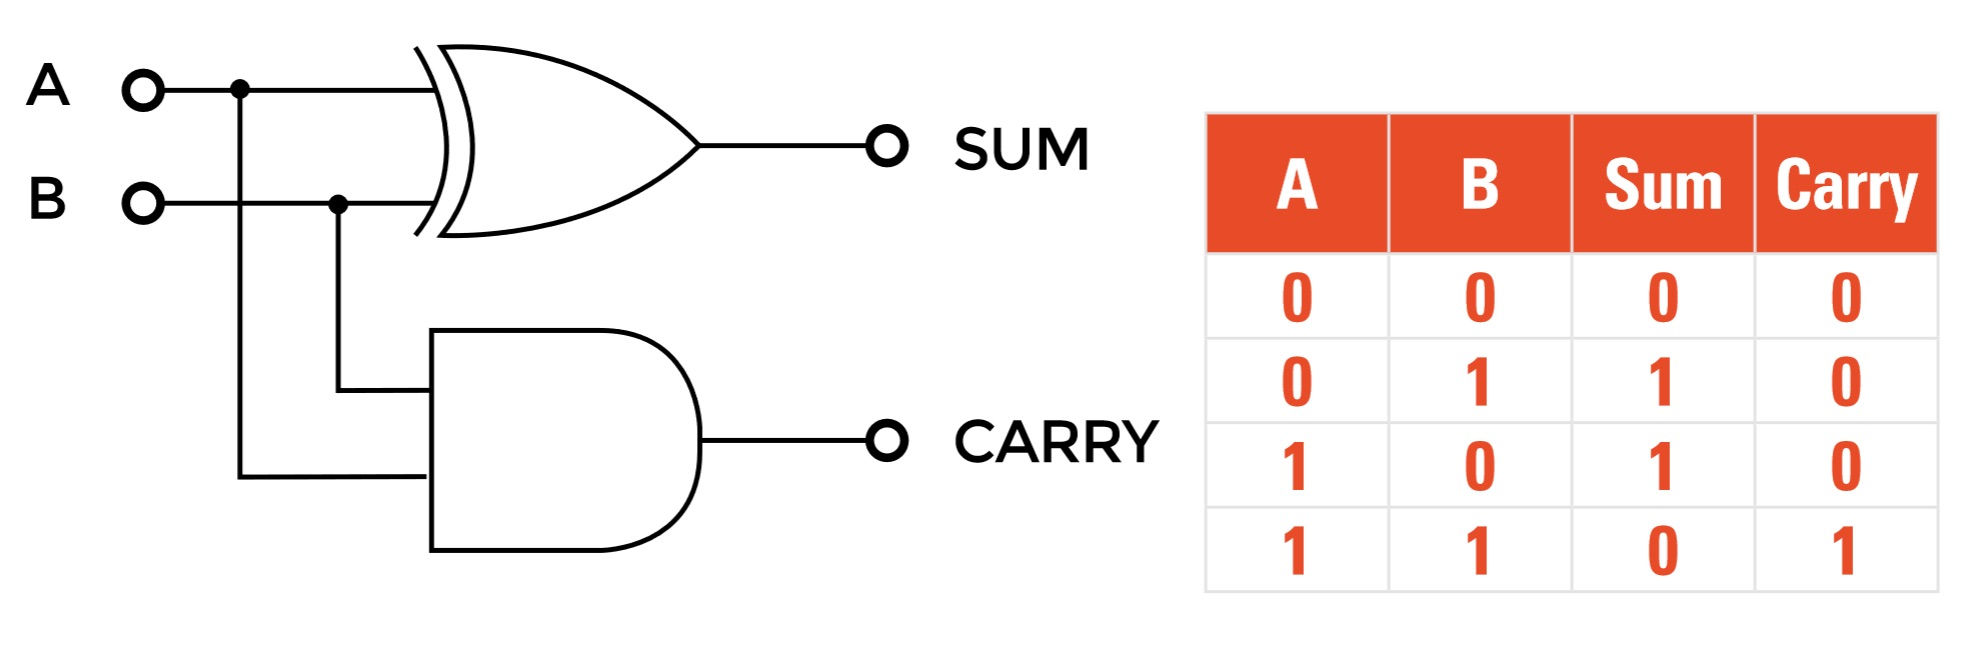
\includegraphics[width=0.7\textwidth]{images/adder.jpeg}
    \caption{A logic diagram of a binary half adder, including truth table output for all possible input combinations. \cite{adder}}\label{fig:ADDER}
\end{figure}

 The ability to implement gates and process bits using them, is a fundamental pillar of computation whether that be classical or quantum. The report will know introduce concepts from quantum physics which are core to understanding how to build a quantum computer. With this knowledge, it will then be possible to draw analogies between classical and quantum computing implementations.

\subsection{Relevant Quantum Physics}

Quantum computing's advantages are a direct result of the quantum mechanical properties such as superposition and entanglement that distinguish it from classical computers. 
These two properties along with quantum teleportation and the Bell inequality will be discussed.
Finally decoherence times of quantum states will be introduced as a means of demonstrating the difficulty with scailability in quantum computing. 


\subsubsection{Superposition}
Superposition is a quantum mechanical phenomenon where an object may exist in multiple states at once. 
For example an electron may be said to be in two places at once - or more accurately its probability function covers multiple areas in space. \cite{noauthor_whatCal_nodate}

Superposition can be observed in the polarisation of light. 
Light can be horizontally, vertically and circularly polarized and much of the light around us is a superposition of the three.
However when light interacts with surfaces their properties can change such as light reflecting off a pond being horizontally polarized. 
Using a linear polariser one can control the direction of polarisation of the light passing through it.
Constructing two polarisers at right angles (horizontal and vertical respectively) one would expect only horizontal polarised light to emitted from the first and then no light to be emitted from the second polariser. 
This is what is experimentally observed - however if a third polariser is placed between the horizontal and vertical polarisers orientated at 45$^\circ$ (as in figure \ref{fig:polarisers}) from both then light will now be transmitted through the final horizontal polariser (at 50$\%$ intensity). \cite{noauthor_whatCal_nodate}
This also emphasises this highly probabilistic behavior of QM where after exiting the second polariser the light is in a superposition of the states which allow diagonal polarisation - some of which is vertical and therefore can pass through the final filter.
\begin{figure}[H]
  \centering
  \begin{subfigure}[t]{0.4\textwidth}
    \centering
    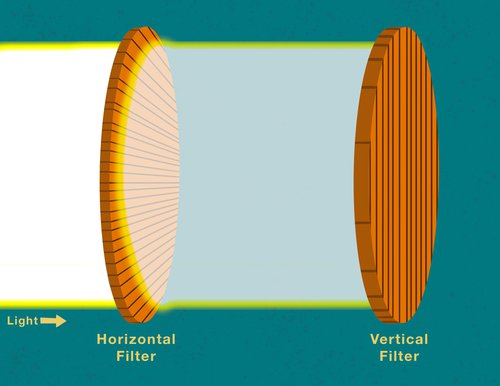
\includegraphics[width=\textwidth]{images/2 polariser.jpg}
    \caption{Unpolarised light passing through a horizontal and then failing to pass through a vertical polarising filter.}\label{fig:2 polarise}
  \end{subfigure}
  \begin{subfigure}[t]{0.4\textwidth}
    \centering
    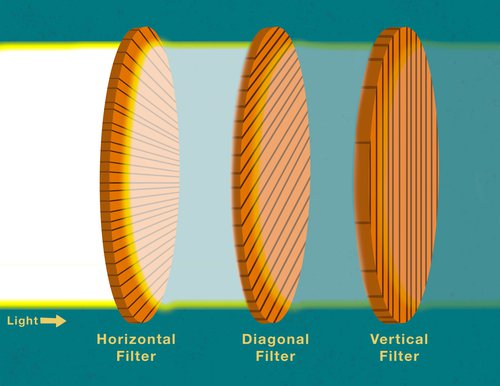
\includegraphics[width=\textwidth]{images/3 polariser.jpg}
    \caption{Unpolarised light passing through three successive polarising filters. A horizontal and vertical filter and a linear polariser orientated 45$^\circ$ between both. }\label{fig:3 polarise}
  \end{subfigure}
  \caption{Unpolarised light passing through linear polarising filters in two set ups. \cite{noauthor_whatCal_nodate}}
  \label{fig:polarisers}
\end{figure}

It is this superposition of states which allows a single qubit to trial multiple values at once. \cite{sonialopezbravo_understanding_nodate}


\subsubsection{Entanglement}
Entanglement is a uniquely quantum mechanical phenomenon where the measurement of one particle's state will effect the state of another particle.
I.e. for interacting states A and B their combined wavefunction cannot be expressed as the product of the individual wavefunctions of A and B if states A and B are entangled. \cite{bransden_quantum_2000}

For example the LHS of equation \ref{eqn:superqubit} is not an entangled system (simply a superposition of states) as it can be expressed as the tensor product of both wavefunctions.

\begin{equation}\label{eqn:superqubit}
    |0\rangle_\phi|0\rangle_\psi + |0\rangle_\phi|1\rangle_\psi + |1\rangle_\phi|0\rangle_\psi +
    |1\rangle_\phi|1\rangle_\psi = |\phi\rangle \otimes |\psi\rangle
\end{equation}

However the system in equation \ref{eqn:entqubit} is entangled as the total system cannot be expressed as a product of the two single systems. 
\begin{equation}\label{eqn:entqubit}
    |0\rangle_\phi|0\rangle_\psi + 
    |1\rangle_\phi|1\rangle_\psi
\end{equation}



Although progress has been made in studying quantum entanglement, there is no complete theory to explain it. 
It does play an integral role in quantum computing however and deeper investigation of it and how to manipulate this property is likely to lead to further applications. \cite{nielsen_quantum_2010}



\subsubsection{Decoherence of States}
Decoherence is when a quantum state collapses into a single state i.e. no longer a superposition.
This is a consideration in quantum computing as qubits are fragile and decoherence may occur - it is especially challenging when trying to scale up to large multi-qubit operations and maintain control over the system. \cite{zhang_observation_2017}
Quantum systems can have a `lifetime', $T_2$ after which the state `relaxes' into a classical single state. 
Therefore a good physical system for quantum computing must have a long $T_2$ and have operations (gates) which are unlikely to cause decoherence. \cite{nielsen_quantum_2010}



\subsection{Quantum Computing}
\subsubsection{Qubits}
Following the general introduction of a qubit in the introduction, a qubit is the quantum form of a classical bit. 
A classical bit can either hold the value of 0 or 1 while a qubit is a superposition of both $|0\rangle$ and $|1\rangle$ as seen in equation \ref{eqn:qubit}
\begin{equation}\label{eqn:qubit}
    |\psi\rangle = \alpha|0\rangle + \beta|1\rangle
\end{equation}
where $\alpha$ and $\beta$ are complex numbers such that $|\alpha|^2 + |\beta|^2 = 1$.
Operations can be preformed on this superposition state and only once the qubit has been measured the state will collapse to either $|0\rangle$ or $|1\rangle$. \cite{nielsen_quantum_2010}
The matrix representations of the $|0\rangle$ and $|1\rangle$ states can be seen in equation \ref{eqn:qmatrix} and is useful for understanding gate operations.

\begin{equation}\label{eqn:qmatrix}
    |0\rangle = \begin{bmatrix}
1 \\
0 
\end{bmatrix} \text{ and } |1\rangle = \begin{bmatrix}
0 \\
1 
\end{bmatrix}  
\end{equation}

Qubits can also be represented as a vector within a radius 1 bloch sphere and represented by angles $\theta$ and $\phi$ as opposed to the complex numbers $\alpha$ and $\beta$, see equation {eqn:bloch}

\begin{equation}\label{eqn:bloch}
    |\psi \rangle = \cos \frac{\theta}{2}|0\rangle + e^{i \phi}\sin \frac{\theta}{2} |1\rangle
\end{equation}

The visual representation of a Bloch sphere can be seen in figure \ref{fig:bloch}.
This is a particularly helpful way of visualising qubits with regards to gate operations as they can be seen as rotations and reflections within this sphere. \cite{noauthor_representing_nodate}


\begin{figure}[H]
    \centering
    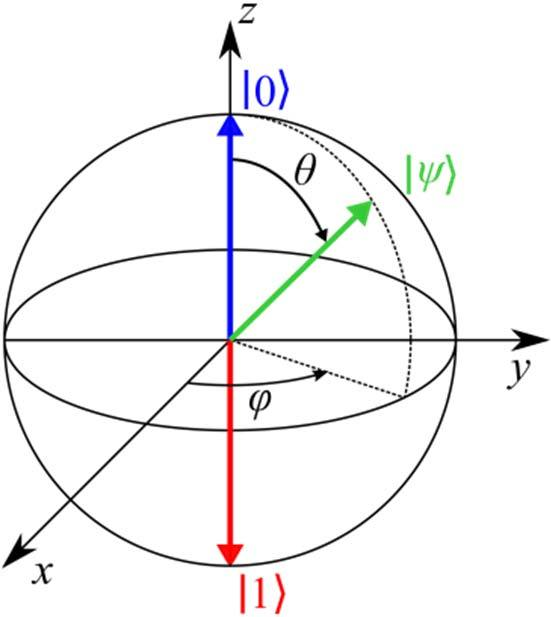
\includegraphics[scale=0.3]{images/Bloch-sphere-representation-of-a-qubit.png}
    \caption{Diagram of a Bloch sphere - 
 representing a qubit as a vector. x-axis is $\frac{|0\rangle + |1\rangle}{\sqrt{2}}$ and y-axis is $\frac{|0\rangle+i|1\rangle}{\sqrt{2}}$.\cite{sebastiano_cryo-cmos_2017}}.\label{fig:bloch}
\end{figure}

As with classical computing, quantum computing requires gates to preform basic manipulation of qubits. 
Calculations are then preformed by using these gates in series.
Quantum gates must be able to modify the probabilities without decoherence or collapse of the wavefunction. 
In the next sections, a selection of common single and two qubit gates are introduced.
The universal set of quantum gates is explained which can be comprised of the gates in section \ref{sec:singlequbit} and \ref{sec:twoqubit}  

\subsubsection{Single Qubit Gates}\label{sec:singlequbit}
Single qubit gates are ones which act on only one qubit. 
This section will describe the Hadamard, Phase Gate and the three Rotation gates. 

{\bf Hadamard gate} is represented as a rotation about the y-axis of 90$^\circ$ and x-axis of 180$^\circ$ of figure \ref{fig:bloch}.
The matrix representation of this is in equation \ref{eqn:hadamard}. i.e. it turned the $|0\rangle$ state into a equal superpostion of $|0\rangle$ and $|1\rangle$

\begin{equation}\label{eqn:hadamard}
    H = \frac{1}{\sqrt{2}} \begin{bmatrix}
1 & 1 \\
1 & -1 
\end{bmatrix}  
\end{equation}
The effect of this gate on a qubit is seen in equation \ref{eqn:qH}
\begin{equation}\label{eqn:qH}
    \left( \alpha \begin{bmatrix}
1 \\
0 
\end{bmatrix}  + \beta  \begin{bmatrix}
0 \\
1 
\end{bmatrix}   \right) \cdot \frac{1}{\sqrt{2}} \begin{bmatrix}
1 & 1 \\
1 & -1 
\end{bmatrix} = \alpha \frac{|0\rangle +|1\rangle}{\sqrt{2}} + \beta \frac{|0\rangle - |1\rangle}{\sqrt{2}}
\end{equation}


{\bf Phase gate} is 
The matrix representation of this is in equation \ref{eqn:phase}
\begin{equation}\label{eqn:phase}
    P =  \begin{bmatrix}
1 & 0 \\
0 & e^{i \phi}
\end{bmatrix}  
\end{equation}


\subsubsection{Two Qubit Gates}\label{sec:twoqubit}
CNOT

\subsubsection{The Universal Set of Quantum Gates}
As in classical computing, quantum algorithms are executed as qubits are passed through and manipulated by a series of consecutive gates. 

The state in equation \ref{eqn:entqubit} (with a factor of $1/\sqrt{2}$ is an interesting illustration of this; it is known as the Bell state, which is 2 qubit entanglement frequently used in quantum computations. The Bell state is formed by applying a Hadamard gate to a qubit, which then acts as a control input for a CNOT gate. The CNOT is applied to this control and another, target, qubit. \cite{mermin_quantum_2007} 
By measuring one of the qubits in the Bell state, one can then reveal the state of the other qubit. If a $|0\rangle$ is measured then the other qubit must be $|0\rangle$ and vice versa. The probability of measuring $|0\rangle$ is 50$\%$ and similarly for measuring $|1\rangle$. 

There are many quantum gates beyond those described so far, including the Toffoli, Controlled-Z and more. However, it can be mathematically proven that a small subset of the quantum gates can be combined to make any of the others. This is known as a universal set. Therefore, a physical quantum computer needs only to implement all of the gates in this set, in order to guarantee that any desired computation is attainable \cite{universalset}.

There is no one universal set of quantum gates, and the choice of which gates to implement is likely dependent on the kinds of calculations the computer will be used for, as well as the practicality given a choice of technology. However, to provide an example, the most commonly used universal set of quantum gates is composed of the CNOT, phase gate and the rotation gates.

\begin{equation}
    Universal\ Set = \{ R_x, R_y, R_z, Ph, CNOT \}
\end{equation}

In fact, it is only necessary to use two of the three rotation gates.

\subsubsection{The DiVincenzo Criteria}
In 2000, the components of a quantum computer, which are introduced in the sections above, were formalised into the DiVincenzo criteria. These are a list of seven objectives that must be fulfilled in order to construct a physical quantum computer. This report will not focus on the final two criteria as they are only necessary for quantum communication, rather than computation \cite{bergou_quantum_2021}.

The report will show how possible technologies for implementing a quantum computer are able to satisfy the following five DiVincenzo criteria.
\begin{enumerate}
    \item Scalability with well defined qubits
    \item The ability to initialise the system in a well defined, determinate state
    \item The ability to read out qubit state with high accuracy
    \item A set of universal quantum gates
    \item Long relevant decoherence times
    \newcounter{enumTemp}
    \setcounter{enumTemp}{\theenumi}
\end{enumerate}

The first objective requires qubits to be in a superposition of two clearly defined states. For example, as a superposition of vertical and horizontal polarisation of light. The greater challenge in the first criterion is that of scalability; in order to unlock the power of quantum computing, it is necessary to have many entangled qubits operating on the same problem.

The second objective is to initialise the qubits into a well defined determinate state i.e. initialise the qubit register so all are in the 0 state $\vert 0\rangle \vert 0\rangle$...$\vert 0 \rangle$. \cite{lapierre_divincenzo_2021}

The third objective is to read out qubit state $\vert 0\rangle$ or $\vert 1 \rangle$ with high accuracy. Measurement that have a higher propbability of error can be repeated in order to mitigate this effect.

The fourth objective is to implement a universal set of gates, as explained above. If an implementation includes all gates in a universal set, then such a computer could emulate any sequence of quantum gates, thus executing any desired  quantum algorithm. This is in many ways a positive simplification for building a quantum computer, as it only requires the assembler to create a few important gates. 

The final objective is for long `relevant' decoherence times; this requires the qubit to stay in a superposition for longer than the duration of gate operations before the state collapses. Without this condition, there would not be a long enough time for taking useful measurements.